\documentclass{standalone}
\usepackage{tikz}
\usepackage{pgfmath}
\usetikzlibrary{arrows.meta}
\tikzset{>={Latex[width=1.5mm,length=1.5mm]}}

\definecolor{darkgreen}{rgb}{0.0, 0.2, 0.13}

\def\levelSize{{1,4,2,3,12,5,6,5,4,3,9,2,8,4,11,2,4}}
\def\levelGroupSize{{7,20,15,14,23,6}}
\def\levelGroupColor{{"red","blue","red","blue","red","blue"}}
\def\diff{{-8,6.7,0,0.7,8,-7.3}}
\def\color{{"red","red","red","blue","blue","blue","red","red","red","blue","blue","blue","red","red","red","blue","blue"}}
\def\Tptr{{0,3,6,9,12,15,17}}

\def\mr{15}
\def\mb{13.3}
\def\var{37.78}
\begin{document}
	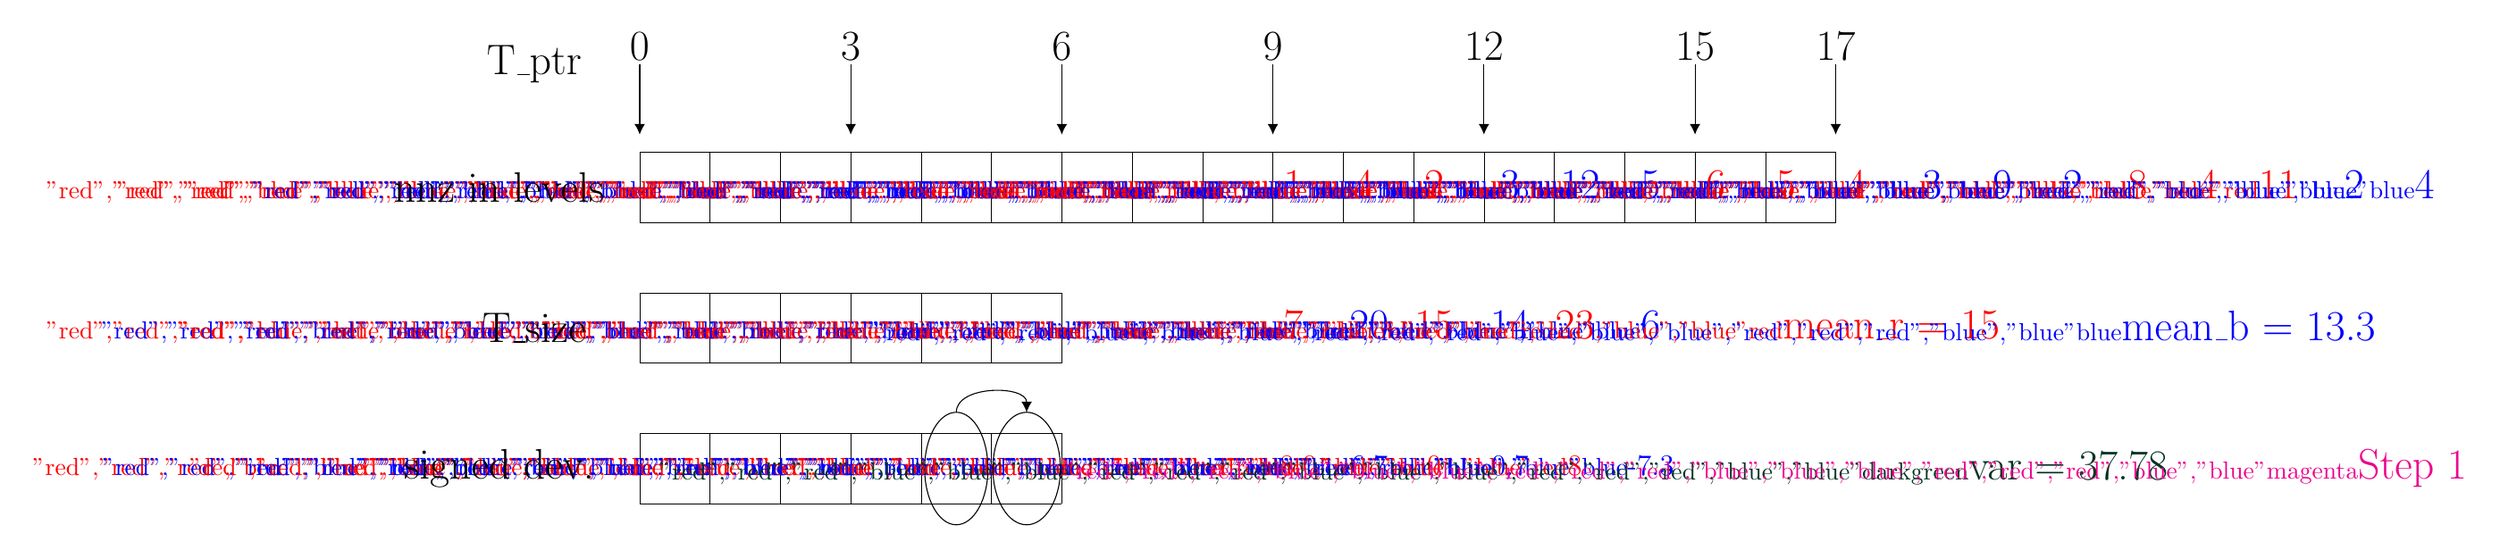
\begin{tikzpicture}

	%	\draw[step=cm,gray,very thin] (0,4) grid (17,5);
		\foreach \x in {0,...,6}
		{
			\pgfmathparse{\Tptr[\x]}
			\edef\currLS{\pgfmathresult}
			\node at (\currLS,4.5) {\LARGE{\currLS}};
			\draw[->] (\currLS,4.25) -- (\currLS,3.25);
		}

	
		\draw[step=1cm,gray,very thin] (0,2) grid (17,3);
		\foreach \x in {0,...,16}
		{
			\pgfmathparse{\levelSize[\x]}
			\edef\currLS{\pgfmathresult}
			\pgfmathparse{\color[\x]}
			\edef\currCOLOR{\pgfmathresult}
			\node[\currCOLOR] at (0.5+\x,2.5) {\LARGE{\currLS}};
		}
	
				

		\draw[step=1cm,gray,very thin] (0,0) grid (6,1);
		\foreach \x in {0,...,5}
		{
			\pgfmathparse{\levelGroupSize[\x]}
			\edef\currLS{\pgfmathresult}
			\pgfmathparse{\levelGroupColor[\x]}
			\edef\currCOLOR{\pgfmathresult}
			\node[\currCOLOR] at (0.5+\x,0.5) {\LARGE{\currLS}};
		}
		
		\node[red] at (9,0.5) {\LARGE{mean\_r = \mr}};
		\node[blue] at (14,0.5) {\LARGE{mean\_b = \mb}};
		
		\draw[step=1cm,gray,very thin] (0,-2) grid (6,-1);
		\foreach \x in {0,...,5}
		{
			\pgfmathparse{\diff[\x]}
			\edef\currLS{\pgfmathresult}
			\pgfmathparse{\levelGroupColor[\x]}
			\edef\currCOLOR{\pgfmathresult}
			\node[\currCOLOR] at (0.5+\x,-1.5) {\large{\currLS}};
		}
		
		\node[darkgreen] at (11,-1.5) {\LARGE{var = \var}};
		
		\draw (5.5,-1.5) ellipse (0.48 and 0.8);
		\draw (4.5,-1.5) ellipse (0.45 and 0.8);
		\draw[->] (4.5,-0.7) to [out=90,in=90] (5.5,-0.7);
		
		\node at (-1.5,4.25) {\LARGE{T\_ptr}};
		\node at (-2,2.5) {\LARGE{nnz in levels}};
		\node at (-1.5,0.5) {\LARGE{T\_size}};	
		\node at (-2,-1.5) {\LARGE{signed dev.}};
		\node[magenta] at (16,-1.5) {\LARGE{Step 1}};	
	\end{tikzpicture}
\end{document}  